\scanpage{30}
\uline{\unsure{Reprenons}}

Considérons un préschéma $X/\mathbb F_p$, et
\diagram{\begin{tikzcd}X & X \arrow[l,"\operatorname{Fr}_X"']\end{tikzcd}}
Comme $\operatorname{Fr}_X$ est un homéo. univ. on conclut que pour un faisceau $F$ sur $X$ et un faisceau $G$ sur $X$ (pour top étale), la donnée de
\diagram{\begin{tikzcd}G \arrow[r,"\alpha"] & \operatorname{Fr}_X^*(F)\end{tikzcd}}
\uline{équivaut} à la donnée de
\diagram{\begin{tikzcd}\operatorname{Fr}_{X*}(G) \arrow[r,"\beta"] & F\end{tikzcd}}
(car $\operatorname{Fr}_{X*}$ et $\operatorname{Fr}_X^*$ sont \inserted{ici} des foncteurs adjoints du côté inhabituel).

Ainsi, la donnée de $\alpha$ définit
\diagram{\begin{tikzcd}\operatorname{Fr}_{X*}(G) \arrow[r,"\operatorname{Fr}_{X*}(\alpha)"] & \operatorname{Fr}_{X*}\operatorname{Fr}_X^*(F) \arrow[r,leftrightarrow,"{\substack{\mathrm{can}^{-1}\\\sim}}"] & F\end{tikzcd}}
et inversement la donnée de $\beta$ définit
\diagram{\begin{tikzcd}G \arrow[r,no head,"{\substack{\mathrm{can}^{-1}\\\sim}}"] & \operatorname{Fr}_X^*\operatorname{Fr}_{X*}(G) \arrow[r,"\operatorname{Fr}_X^*(\beta)"] & \operatorname{Fr}_X^*(F)\end{tikzcd}}
Nous allons \uline{\unsure{fabriquer}} \deleted{\unsure{donc}} des hom qui se correspondent de cette façon\textsuperscript{*} \deleted{et} Nous allons maintenant, pour $F=G$, définir \deleted{\unsure{des}} un hom canonique
\margin{\textsuperscript{*} \unsure{en mettant les barres sur} $\unsure{*}$ \unsure{et} $\unsure{*}$ \unsure{pour distinguer} \unsure{à la fois} \unsure{opérations}.}\margin{\figure{\begin{tikzpicture}\draw (0,0)..controls(-.4,-.25)and(-.4,-.5)..(0,-.55)--(8.7,-.55)..controls(9,-.55)and(9,-.2)..(8.8,.05)..controls(8.1,.5)and(8,.3)..(7.6,.22);\end{tikzpicture}}}
\margin{\figure{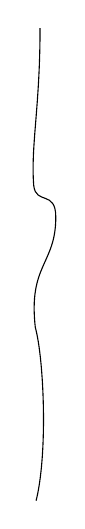
\begin{tikzpicture}[x=1cm,y=1cm]\draw (0,0)..controls(0,-1)and(-.12,-1.5)..(-.08,-2)..controls(-.05,-2.25)and(.2,-2.05)..(.2,-2.4)..controls(.2,-3)and(-.15,-3)..(-.06,-3.8)..controls(.05,-4.2)and(.1,-5.4)..(-.05,-6);\end{tikzpicture}}}
\diagram{\begin{tikzcd}[column sep=large]
(1)\quad F & \operatorname{Fr}_X^*(F) \arrow[l,"\operatorname{Fr}_{F/X}"'] \arrow[l,phantom,"\deleted{\unsure{\rightarrow}}" description]
\end{tikzcd}}\qquad i.e.
\diagram{\begin{tikzcd}[column sep=large]
(2)\quad\operatorname{Fr}_{X*}(F) \arrow[r,"\operatorname{Fr}_{F/X}"] & F
\end{tikzcd}}
(qui est d'ailleurs un isom, mais on voudra l'ignorer dans la plupart des cas !). C'est sous la forme (2) que la définition \unsure{faiscea-}
\mspage{29}
